\documentclass{article}

\usepackage{tikz}
\usetikzlibrary{shapes, arrows.meta, positioning, calc}

\tikzset{
	block/.style = {draw, rectangle, minimum height=1.5em, minimum width=3em, align=center},
	arrow/.style = {->, thick},
}

\begin{document}

\begin{figure*}[htbp]
	%\centering
	\begin{center}
		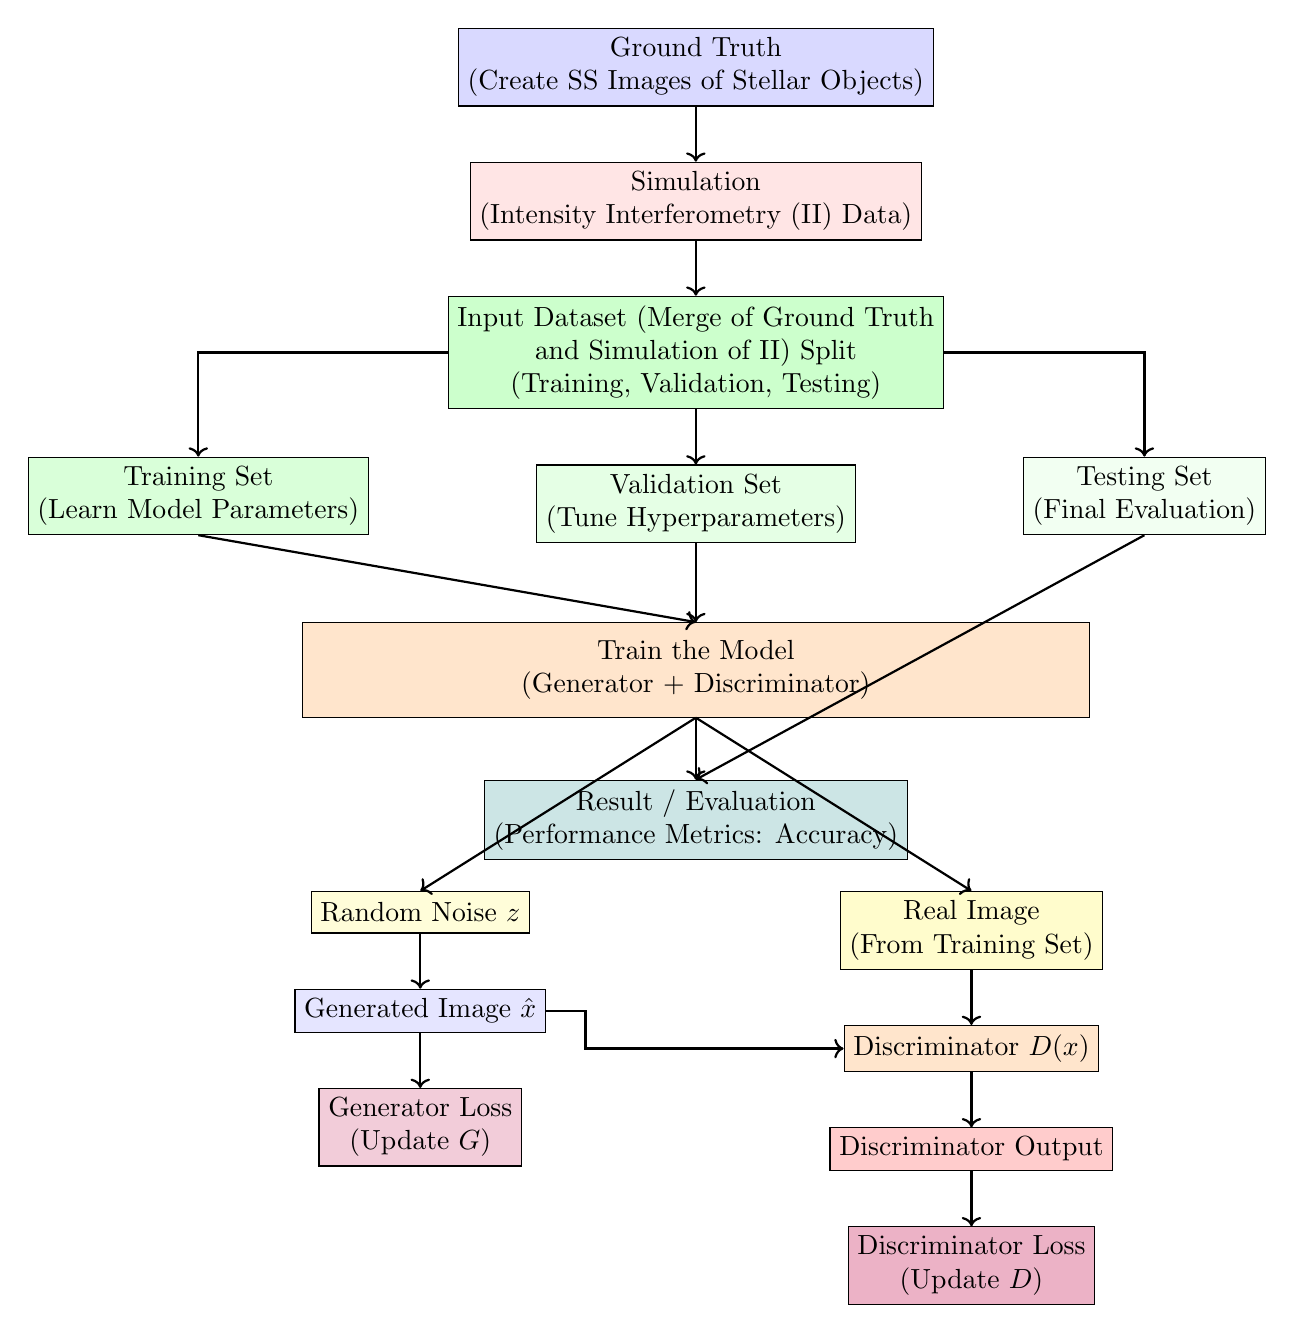
\begin{tikzpicture}[node distance=0.7cm]
			
			% Data pipeline
			\node[block, fill=blue!15] (data) {Ground Truth \\ (Create SS Images of Stellar Objects)};
			\node[block, fill=red!10, below=of data] (pre) {Simulation \\ (Intensity Interferometry (II) Data)};
			\node[block, fill=green!20, below=of pre, minimum width=5cm] (split) {Input Dataset (Merge of Ground Truth \\ and Simulation of II) Split \\ (Training, Validation, Testing)};
			
			% Training, Validation, Testing
			\node[block, fill=green!15, below left=0.6cm and 1.0cm of split] (train) {Training Set \\ (Learn Model Parameters)};
			\node[block, fill=green!10, below=of split] (val) {Validation Set \\ (Tune Hyperparameters)};
			\node[block, fill=green!05, below right=0.6cm and 1.0cm of split] (test) {Testing Set \\ (Final Evaluation)};
			
			% Model training block
			\node[block, fill=orange!20, below= 1.0cm of val, minimum width=10cm, minimum height=1.2cm] (mod) {Train the Model \\ (Generator + Discriminator)};
			
			% Generator side (left)
			\node[block, fill=yellow!15, below=2.2cm of mod, xshift=-3.5cm] (noise) {Random Noise $z$};
			\node[block, fill=blue!10, below=of noise] (gen) {Generated Image $\hat{x}$};
			\node[block, fill=purple!20, below=of gen] (gloss) {Generator Loss \\ (Update $G$)};
			
			% Discriminator side (right)
			\node[block, fill=yellow!20, below=2.2cm of mod, xshift=+3.5cm] (real) {Real Image \\ (From Training Set)};
			\node[block, fill=orange!20, below=of real] (disc) {Discriminator $D(x)$};
			\node[block, fill=red!20, below=of disc] (out) {Discriminator Output};
			\node[block, fill=purple!30, below=of out] (dloss) {Discriminator Loss \\ (Update $D$)};
			
			% Final result block
			\node[block, fill=teal!20, below= 3cm of val, minimum width=5cm] (res) {Result / Evaluation \\ (Performance Metrics: Accuracy)};
			
			% Connections
			\draw[arrow] (data) -- (pre);
			\draw[arrow] (pre) -- (split);
			%\draw[arrow] (split.south west) |- (train.north);
			\draw[arrow] (split.west) -| (train.north);
			\draw[arrow] (split.south) -- (val.north);
			\draw[arrow] (split.east) -| (test.north);
			\draw[arrow] (train.south) -- (mod.north);
			
			%Newly Introduced Connections (S Sarangi)
			\draw[arrow] (val.south) -- (mod.north);
			\draw[arrow] (mod.south) -- (res.north);
			
			% GAN arrows
			\draw[arrow] (mod.south) -- (noise.north);
			\draw[arrow] (mod.south) -- (real.north);
			\draw[arrow] (noise.south) -- (gen.north);
			\draw[arrow] (gen.south) -- (gloss.north);
			\draw[arrow] (real.south) -- (disc.north);
			\draw[arrow] (gen.east) -- ++(0.5,0) |- (disc.west);
			\draw[arrow] (disc.south) -- (out.north);
			\draw[arrow] (out.south) -- (dloss.north);
			
			% Validation & Testing to Result
			%\draw[arrow] (val.south) -- (res.north);
			\draw[arrow] (test.south) -- (res.north);
			
		\end{tikzpicture}
	\end{center}
\caption{A block diagram for the process of image reconstruction through GAN.}
\end{figure*}

\end{document}
